%Here we want to illustrate the reasons why conditional support in existing data flow analyses is too restricted and why support for model checking is not appropriate.

%We should do it by way of examples and introduce the concepts and advantages of our proposed approaches.

%Show a general analysis.\\
Before introducing conditional data-flow analysis we would like to start with an example of a traditional data-flow analysis. Data-flow analysis calculates some information for each point in a program based on the program structure and  the language semantics. The calculated facts then later used to reason about program properties. One type of property that we consider in this work is safety property. A safety property $\varphi$ is a fact about the program that must hold on all feasible program executions. The type of data-flow analyses that able to determine properties that are satisfied by all paths are called {\em must} analyses. Commonly used safety properties are program assertions and we going to assume them in our further discussions.

Consider a program and its corresponding control flow graph (CFG) on Figure~\ref{fig:programExample}. In this example x and y are variables of the integer type and the edges of CFG are labeled with $T$ for {\em true} branches and $F$ for {\em false} branches of conditional statements. In this example we want to use a data-flow analysis to verify that the assertion at the label $b_4$ holds. In CFG we ``desugare'' the assertion into a conditional statement. 

\begin{figure}[!t]
\begin{minipage}[b]{0.20\textwidth}
\small
\begin{lstlisting}
b1: if (x > 0){
          y = x;
          x = 0; 
      } 

b2: if(x > 0){
          x = -x;
b3: } else if (y == 0){
           x = 1;
      }
b4: assert(x == 0);
\end{lstlisting}
\end{minipage}
~
\begin{minipage}{0.20\textwidth}
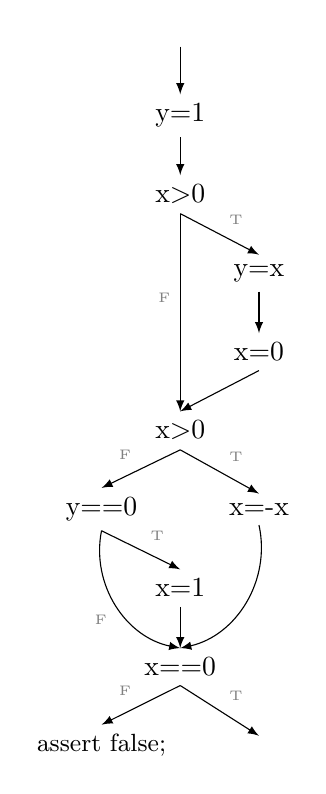
\begin{tikzpicture}[>=latex]
\node[name=enter]{};
\node[name=stmt_1, below of=enter]{y=1};
\node[name=if_1, below of=stmt_1]{x$>$0};
\node[name=if_1_body_1, below of=if_1, xshift=10mm]{y=x};
\node[name=if_1_body_2, below of=if_1_body_1]{x=0};
\node[name=if_2, below of=if_1_body_2, xshift=-10mm]{x$>$0};
\node[name=if_2_true, below of=if_2, xshift=10mm]{x=-x};
\node[name=if_3, below of=if_2, xshift=-10mm]{y==0};
\node[name=if_3_true, below of=if_3, xshift=10mm]{x=1};
\node[name=assert, below of=if_3_true]{x==0};
\node[name=exit, below of=assert, xshift=10mm] {};
\node[name=assertFalse, below of=assert, xshift=-10mm] {\small assert false;};

\draw(enter.south) edge[->](stmt_1.north);
\draw(stmt_1.south) edge[->](if_1.north);
\draw(if_1.south) edge[->]node[above right]{\tiny {\color{gray}T}}(if_1_body_1.north);
\draw(if_1_body_1.south) edge[->](if_1_body_2.north);
\draw(if_1_body_2.south) edge[->](if_2.north);
\draw(if_1.south) edge[->]node[above left]{\tiny {\color{gray}F}}(if_2.north);
\draw(if_2.south) edge[->]node[above right]{\tiny {\color{gray}T}}(if_2_true.north);
\draw(if_2.south) edge[->]node[above left]{\tiny {\color{gray}F}}(if_3.north);
\draw(if_3.south) edge[->]node[above right]{\tiny {\color{gray}T}}(if_3_true.north);
\draw(if_3_true.south) edge[->](assert.north);
\draw(if_3.south) edge[->, bend right=45]node[below left]{\tiny {\color{gray}F}}(assert.north);
\draw(if_2_true.south) edge[->, bend right=-45](assert.north);
\draw(assert.south) edge[->]node[above left]{\tiny {\color{gray}F}}(assertFalse.north);
\draw(assert.south) edge[->]node[above right]{\tiny {\color{gray}T}}(exit.north);

\end{tikzpicture}
\end{minipage}
\caption{Program example: source code and the corresponding CFG}
\label{fig:programExample}
\end{figure}

To verify the assertion we employ {\em zero} data-flow analysis whose abstract domain is defined by the set $\{\bot, 0, \neg 0, \top\}$. Where $\bot$ element represents the empty set of concrete values; $0$ -- the singleton set $\{0\}$ of concrete values, $\neg 0$ -- any concrete value except $0$ and $\top$ -- any concrete value. The left CFG on Figure~\ref{fig:analysisExample} shows the result of zero analysis where each edge is annotated with a tuple containing abstract values for x and y variables respectively. Clearly the analysis fails to verify $\varphi$ since it cannot prove that the false branch of x$==$0 condition is infeasible, i.e., the value of x or y is not $\bot$.

%How it can be more precise when it is changed to conditional.\\
One of the main reasons why data-flow analysis fails to verify $\varphi$ is the over-approximation that takes place when variable values from different paths are merged. For example, before the merge point the value of x on the true branch of $b_1$ is $0$ which is safely over-approximated by $\top$ at the merge point with the false branch of $b_1$. Thus, to improve the precision of data-flow analysis we need to restrict the set of paths it analyzes. It can be done by either restricting entry values of variables or by explicitly specifying the set of paths to be analyzed. We refer to the former as predicate-based condition and the latter as path-based condition.

%Now consider a case when the analysis has restricted the input domain of x to $0$ value. Then as shown on the middle left of Figure~\ref{fig:analysisExample} the analysis was able to determine that the assertion is not violated under that condition. Thus conditional analysis with the constraint $\phi :=$ x=$0 \land$ y = $\top$ are able to verify the program.

To illustrate conditional data-flow analysis with predicate-based we use the previous zero analysis and restrict the entry value of x  to the abstract domain element $0$. The result of such conditional analysis is shown on middle left CFG of Figure~\ref{fig:analysisExample}. The picture shows that condition was able to increase the precision of zero analysis since the analysis was able to verify the program for the entry value x$=0$.

Obviously in order to make the verification unconditional the analysis must also show that $\varphi$ also holds for the condition complement, i.e., when they entry value of x is $\neg 0$. The middle right CFG that on the same figure shows that as in the case of the original analysis the result is inconclusive. Thus conditions expressed as predicates over the input values not necessarily improve data-flow analysis precision.

To illustrate conditional data-flow analysis with path-based condition we restrict zero analysis to propagate program facts along the true branch of $b_1$ while skipping its false branch. The right CFG on Figure~\ref{fig:analysisExample} depicts the result of such conditional analysis. Once again conditional zero analysis was able to determine that all program paths following the true outcome of $b_1$ do not violate $\varphi$. Yet when the analysis is restricted to only the false branch of $b_1$ the result becomes inconclusive again.

\begin{figure*}[t]
\begin{minipage}{0.22\textwidth}
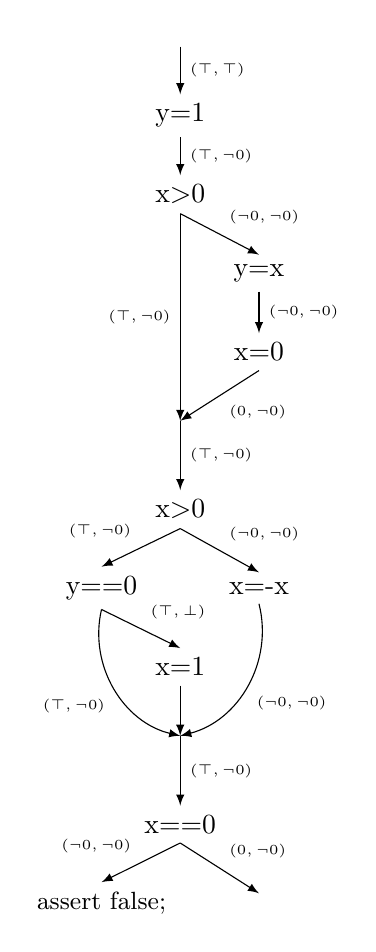
\begin{tikzpicture}[>=latex]
\node[name=enter]{};
\node[name=stmt_1, below of=enter]{y=1};
\node[name=if_1, below of=stmt_1]{x$>$0};
\node[name=if_1_body_1, below of=if_1, xshift=10mm]{y=x};
\node[name=if_1_body_2, below of=if_1_body_1]{x=0};
\node[name=if_1_merge, below of=if_1_body_2, xshift=-10mm]{};
\node[name=if_2, below of=if_1_merge]{x$>$0};
\node[name=if_2_true, below of=if_2, xshift=10mm]{x=-x};
\node[name=if_3, below of=if_2, xshift=-10mm]{y==0};
\node[name=if_3_true, below of=if_3, xshift=10mm]{x=1};
\node[name=if_2_merge, below of=if_3_true]{};
\node[name=assert, below of=if_2_merge]{x==0};
\node[name=exit, below of=assert, xshift=10mm] {};
\node[name=assertFalse, below of=assert, xshift=-10mm] {\small assert false;};

\draw(enter.south) edge[->]node[right]{\tiny $(\top,\top)$}(stmt_1.north);
\draw(stmt_1.south) edge[->]node[right]{\tiny $(\top,\neg 0)$}(if_1.north);
\draw(if_1.south) edge[->]node[above right]{\tiny $(\neg 0, \neg 0)$}(if_1_body_1.north);
\draw(if_1_body_1.south) edge[->]node[right]{\tiny $(\neg 0,\neg 0)$}(if_1_body_2.north);
\draw(if_1_body_2.south) edge[->]node[below right]{\tiny $(0,\neg 0)$}(if_1_merge.north);
\draw(if_1.south) edge[->]node[left]{\tiny $(\top,\neg 0)$}(if_1_merge.north);
\draw(if_1_merge.north) edge[->]node[right]{\tiny $(\top, \neg 0)$}(if_2.north);
\draw(if_2.south) edge[->]node[above right]{\tiny $(\neg 0, \neg 0)$}(if_2_true.north);
\draw(if_2.south) edge[->]node[above left]{\tiny $(\top,\neg 0)$}(if_3.north);
\draw(if_3.south) edge[->]node[above right]{\tiny $(\top, \bot)$}(if_3_true.north);
\draw(if_3_true.south) edge[->](if_2_merge.north);
\draw(if_3.south) edge[->, bend right=45]node[below left]{\tiny $(\top, \neg 0)$}(if_2_merge.north);
\draw(if_2_true.south) edge[->, bend right=-45]node[below right]{\tiny $(\neg 0, \neg 0)$}(if_2_merge.north);
\draw(if_2_merge.north) edge[->]node[right]{\tiny $(\top,\neg 0)$}(assert.north);
\draw(assert.south) edge[->]node[above left]{\tiny $(\neg 0, \neg 0)$}(assertFalse.north);
\draw(assert.south) edge[->]node[above right]{\tiny $(0, \neg 0)$}(exit.north);
\end{tikzpicture}
\end{minipage}
~
\begin{minipage}{0.22\textwidth}
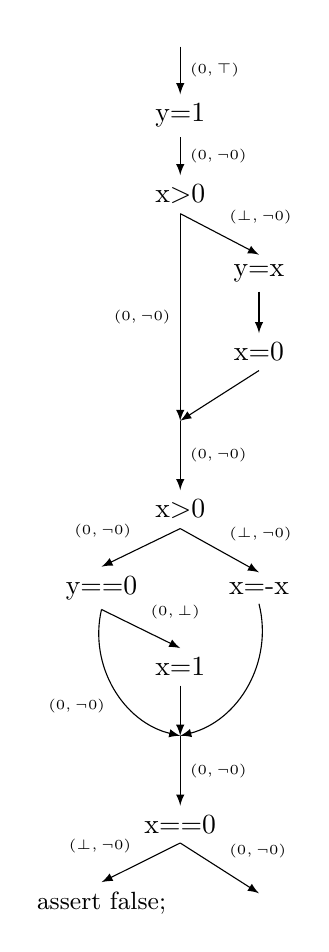
\begin{tikzpicture}[>=latex]
\node[name=enter]{};
\node[name=stmt_1, below of=enter]{y=1};
\node[name=if_1, below of=stmt_1]{x$>$0};
\node[name=if_1_body_1, below of=if_1, xshift=10mm]{y=x};
\node[name=if_1_body_2, below of=if_1_body_1]{x=0};
\node[name=if_1_merge, below of=if_1_body_2, xshift=-10mm]{};
\node[name=if_2, below of=if_1_merge]{x$>$0};
\node[name=if_2_true, below of=if_2, xshift=10mm]{x=-x};
\node[name=if_3, below of=if_2, xshift=-10mm]{y==0};
\node[name=if_3_true, below of=if_3, xshift=10mm]{x=1};
\node[name=if_2_merge, below of=if_3_true]{};
\node[name=assert, below of=if_2_merge]{x==0};
\node[name=exit, below of=assert, xshift=10mm] {};
\node[name=assertFalse, below of=assert, xshift=-10mm] {\small assert false;};

\draw(enter.south) edge[->]node[right]{\tiny $(0,\top)$}(stmt_1.north);
\draw(stmt_1.south) edge[->]node[right]{\tiny $(0,\neg 0)$}(if_1.north);
\draw(if_1.south) edge[->]node[above right]{\tiny $(\bot, \neg 0)$}(if_1_body_1.north);
\draw(if_1_body_1.south) edge[->](if_1_body_2.north);
\draw(if_1_body_2.south) edge[->](if_1_merge.north);
\draw(if_1.south) edge[->]node[left]{\tiny $(0,\neg 0)$}(if_1_merge.north);
\draw(if_1_merge.north) edge[->]node[right]{\tiny $(0, \neg 0)$}(if_2.north);
\draw(if_2.south) edge[->]node[above right]{\tiny $(\bot, \neg 0)$}(if_2_true.north);
\draw(if_2.south) edge[->]node[above left]{\tiny $(0,\neg 0)$}(if_3.north);
\draw(if_3.south) edge[->]node[above right]{\tiny $(0, \bot)$}(if_3_true.north);
\draw(if_3_true.south) edge[->](if_2_merge.north);
\draw(if_3.south) edge[->, bend right=45]node[below left]{\tiny $(0, \neg 0)$}(if_2_merge.north);
\draw(if_2_true.south) edge[->, bend right=-45](if_2_merge.north);
\draw(if_2_merge.north) edge[->]node[right]{\tiny $(0,\neg 0)$}(assert.north);
\draw(assert.south) edge[->]node[above left]{\tiny $(\bot, \neg 0)$}(assertFalse.north);
\draw(assert.south) edge[->]node[above right]{\tiny $(0, \neg 0)$}(exit.north);
\end{tikzpicture}
\end{minipage}
~
\begin{minipage}{0.22\textwidth}
\begin{tikzpicture}[>=latex]
\node[name=enter]{};
\node[name=stmt_1, below of=enter]{y=1};
\node[name=if_1, below of=stmt_1]{x$>$0};
\node[name=if_1_body_1, below of=if_1, xshift=10mm]{y=x};
\node[name=if_1_body_2, below of=if_1_body_1]{x=0};
\node[name=if_1_merge, below of=if_1_body_2, xshift=-10mm]{};
\node[name=if_2, below of=if_1_merge]{x$>$0};
\node[name=if_2_true, below of=if_2, xshift=10mm]{};
\node[name=if_3, below of=if_2, xshift=-10mm]{{\em the rest is the same }};
\node[name=if_3_true, below of=if_3, xshift=10mm]{{\em as on the leftmost graph}};
\node[name=if_2_merge, below of=if_3_true]{};
\node[name=assert, below of=if_2_merge]{};
\node[name=exit, below of=assert, xshift=10mm] {};
\node[name=assertFalse, below of=assert, xshift=-10mm] {};

\draw(enter.south) edge[->]node[right]{\tiny $(\neg 0,\top)$}(stmt_1.north);
\draw(stmt_1.south) edge[->]node[right]{\tiny $(\neg 0,\neg 0)$}(if_1.north);
\draw(if_1.south) edge[->]node[above right]{\tiny $(\neg 0, \neg 0)$}(if_1_body_1.north);
\draw(if_1_body_1.south) edge[->]node[right]{\tiny $(\neg 0, \neg 0)$}(if_1_body_2.north);
\draw(if_1_body_2.south) edge[->]node[below right]{\tiny $(0, \neg 0)$}(if_1_merge.north);
\draw(if_1.south) edge[->]node[left]{\tiny $(\neg 0,\neg 0)$}(if_1_merge.north);
\draw(if_1_merge.north) edge[->]node[right]{\tiny $(\top, \neg 0)$}(if_2.north);

\end{tikzpicture}
\end{minipage}
~
\begin{minipage}{0.22\textwidth}
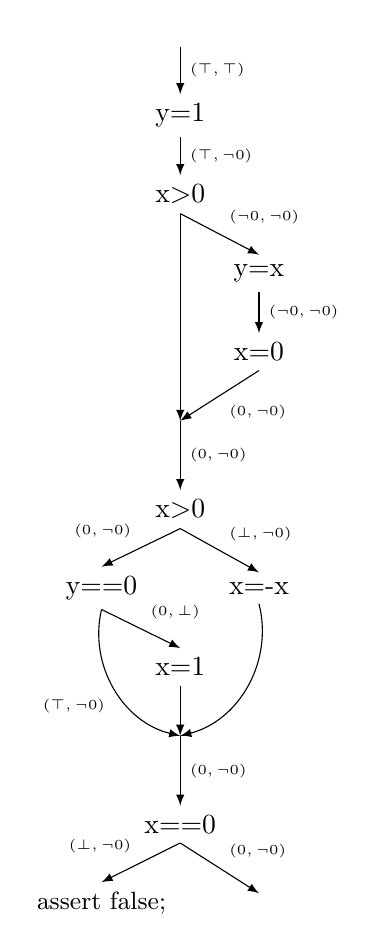
\begin{tikzpicture}[>=latex]
\node[name=enter]{};
\node[name=stmt_1, below of=enter]{y=1};
\node[name=if_1, below of=stmt_1]{x$>$0};
\node[name=if_1_body_1, below of=if_1, xshift=10mm]{y=x};
\node[name=if_1_body_2, below of=if_1_body_1]{x=0};
\node[name=if_1_merge, below of=if_1_body_2, xshift=-10mm]{};
\node[name=if_2, below of=if_1_merge]{x$>$0};
\node[name=if_2_true, below of=if_2, xshift=10mm]{x=-x};
\node[name=if_3, below of=if_2, xshift=-10mm]{y==0};
\node[name=if_3_true, below of=if_3, xshift=10mm]{x=1};
\node[name=if_2_merge, below of=if_3_true]{};
\node[name=assert, below of=if_2_merge]{x==0};
\node[name=exit, below of=assert, xshift=10mm] {};
\node[name=assertFalse, below of=assert, xshift=-10mm] {\small assert false;};

\draw(enter.south) edge[->]node[right]{\tiny $(\top,\top)$}(stmt_1.north);
\draw(stmt_1.south) edge[->]node[right]{\tiny $(\top,\neg 0)$}(if_1.north);
\draw(if_1.south) edge[->]node[above right]{\tiny $(\neg 0, \neg 0)$}(if_1_body_1.north);
\draw(if_1_body_1.south) edge[->]node[right]{\tiny $(\neg 0,\neg 0)$}(if_1_body_2.north);
\draw(if_1_body_2.south) edge[->]node[below right]{\tiny $(0,\neg 0)$}(if_1_merge.north);
\draw(if_1.south) edge[->](if_1_merge.north);
\draw(if_1_merge.north) edge[->]node[right]{\tiny $(0, \neg 0)$}(if_2.north);
\draw(if_2.south) edge[->]node[above right]{\tiny $(\bot, \neg 0)$}(if_2_true.north);
\draw(if_2.south) edge[->]node[above left]{\tiny $(0,\neg 0)$}(if_3.north);
\draw(if_3.south) edge[->]node[above right]{\tiny $(0, \bot)$}(if_3_true.north);
\draw(if_3_true.south) edge[->](if_2_merge.north);
\draw(if_3.south) edge[->, bend right=45]node[below left]{\tiny $(\top, \neg 0)$}(if_2_merge.north);
\draw(if_2_true.south) edge[->, bend right=-45](if_2_merge.north);
\draw(if_2_merge.north) edge[->]node[right]{\tiny $(0,\neg 0)$}(assert.north);
\draw(assert.south) edge[->]node[above left]{\tiny $(\bot, \neg 0)$}(assertFalse.north);
\draw(assert.south) edge[->]node[above right]{\tiny $(0, \neg 0)$}(exit.north);
\end{tikzpicture}
\end{minipage}
\caption{Analysis examples: {\em zero} analysis result (left), conditional {\em zero} analysis result with restricted input domain $x=0$ (middle left), $x=\neg 0$ (middle right), and the restricted set of paths (right).} 
\label{fig:analysisExample}
\end{figure*}

These examples indicate that some predicate and path based conditions posed on data-flow analysis can improve its precision. However, unlike previous work where conditions enabling the best precision can either be determined from the analysis design or during analysis run, for data-flow analysis such conditions cannot be obtained  using methods described in the related work. The section on related work describes in details the reason but in the essence the cause is that data-flow analysis cannot distinguish the source of precision losses which can be due to the over-approximation or due to the analysis design.

Thus the purpose of our work is to investigate what type of conditions, i.e., predicate-based, path-based or their combination, is better fitted to improve the precision of data-flow analysis. In order to obtain a better evaluation we not only compare condition types based on their ability to enable the best precision (like on the middle left and right CFGs of Figure~\ref{fig:analysisExample}) but also based their partial result, i.e., when an analysis can verify $\varphi$ on a subset of analyzed paths. As example consider the original zero analysis on left of Figure~\ref{fig:analysisExample}. Even though the analysis cannot verify $\varphi$ for all paths it can definitely tell that the set of paths containing the true branch of $b_3$ cannot violate $\varphi$ because these paths are infeasible. To represent and compare partial results of conditional data-flow analysis we introduce path language. Using such encoding we can record the partial result of unconditional zero analysis as $*;b_3;*$ and the result of condition zero analysis on the rightmost CFG of Figure~\ref{fig:analysisExample} as $b_1;*$. Section ... explores the paths language in greater details.

Overall our work focuses on answering (empirically) the following research questions:
\begin{enumerate}
\item Does the predicate-based precondition increase the partial output of data-flow analysis?
\item Does the path-based precondition increase the partial output of data-flow analysis?
\item How do the two representations compare with each other?
\item Does the combination of predicate-based and path-based preconditions increase the partial output of data-flow analysis comparing to their separate results.
\end{enumerate}

%Why we cannot determine a priori or during run-time what is needed for a better precision. And why it can be done for model checker and why model checker can always produce answer for the given set of path and why logical characterization is sufficient for it. But the logical characterization is not possible for d.f.a. Because in conditional model checking the predicates are tracked.

%A key here is to crystalize the contributions of the work, e.g., data flow analysis
%\begin{itemize}
%\item requires a new means of encoding conditions -- path languages;
%\item introduces overapproximation when it encounters program structures that are a mismatch for its reasoning engine which makes triggering condition generation more challenging, whereas verification approaches can detect those mismatches syntactically;
%\item something about ``partial analysis results''
%\end{itemize}



